\subsection{Liquid phantom protocol for linearity test}

To evaluate the linearity of fluorescence signal intensity with respect to dye concentration, we conducted liquid phantom experiments for each fluorescent dye. The dyes were imaged in the detection channels corresponding to their peak excitation wavelengths: IR680 and AF700 in the $700$ nm channel and AF750 and IR800 in the $800$ nm channel. IR680 and AF700 were prepared and imaged in a single $96$ well plate, as were AF750 and IR800. For each dye, a series of eight concentrations was prepared, $0.1 nM, 1 nM, 10 nM,  20 nM, 40 nM,60 nM, 80 nM$, and $100 nM$. Each concentration was tested in triplicate, resulting in 24 wells per dye to ensure statistical robustness.

Each well contained a total volume of $300$ µL, composed of $15$ µL of $20\%$ Intralipid, $15$ µL of $20\%$ bovine serum albumin (BSA), a calculated volume of dye stock solution, and PBS to complete the volume. The volume of dye stock required to achieve the final target concentration ( $C_{final}$) was determined using the dilution equation ~\ref{eq:dilution_equation}:

\begin{equation}
    \label{eq:dilution_equation}
    V_{dye} = \frac{C_{final} \cdot V_{final}}{C_{dye}}
\end{equation}

where $V_{dye}$ is the volume of dye stock solution, $C_{final}$ is the desired final concentration, $V_{final}$ is the total
volume of the well, and $C_{dye}$ is the concentration of the dye stock solution. The volume of PBS was adjusted accordingly:

\begin{equation}
    \label{eq:pbs_volume}
    V_{PBS} = V_{final} - V_{dye} - V_{Intralipid} - V_{BSA}
\end{equation}

Three replicate wells containing no dye were included on each plate for background subtraction. The image was taken in the Pearl imaging system, and the resulting fluorescence image was analyzed with ImageJ.

\subsection{Liquid phantom protocol for combination experiments}
Following the determination of the linear response range and the selection of a uniform fluorescence intensity value, we calculated the corresponding dye concentrations that produced this signal within a $300$ µL volume. Each dye was then imaged individually and in binary combinations with dyes from the opposite detection channel, for example, IR680 alone and in combination with AF750 and IR800.

As in the linearity experiments, each well was prepared with a total volume of $300$ µL, including $15$ µL of $20\%$ Intralipid, $15$ µL of $20\%$ BSA, the required volume (s) of the dye stock solution and the volume of PBS. Individual volumes of each dye were calculated using the same dilution equation ~\ref{eq:dilution_equation} and PBS was added to complete the total volume. A schematic of the 
$96$-well plate layout is provided in Figure ~\ref{fig:plate_map}. 


\begin{figure}[H]
    \centering
    \begin{minipage}{0.7\linewidth}
        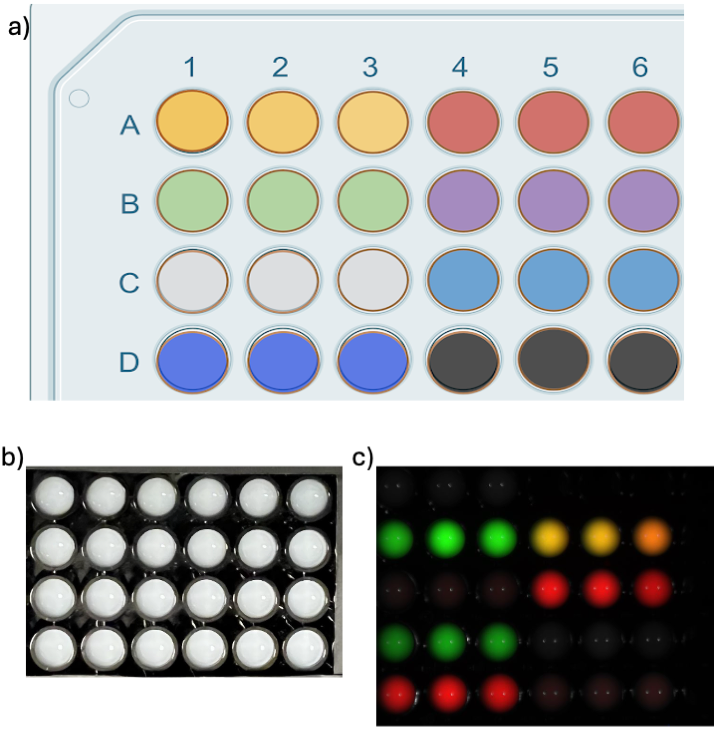
\includegraphics[width=\linewidth]{figures/plate-map.png}
        \captionsetup{justification=raggedright, singlelinecheck=false}
        \caption[Combination experiments set up]{
            \textbf{Combination fluorophore experiments set up.} 
            (a) Plate map showing the layout of dye combinations and controls 
            in a 96-well plate. Wells A1-A3 contain combinations of AF700 with IR800; 
            A4-A6 contain IR680 with IR800. Wells B1-B3 contain AF700 with AF750; 
            B4-B6 contain IR680 with AF750. Row C contains single-agent controls: 
            IR800 (C1-C3) and AF750 (C4-C6). Row D contains IR680 (D1-D3) and AF700 (D4-D6). 
            Wells E1-E3 are dye-free controls. 
            (b) Image of the 96-well plate before imaging. 
            (c) Representative fluorescence image from the Pearl Imaging System showing spectral separation of the fluorophores.
        }
        \label{fig:plate_map}
    \end{minipage}
\end{figure}


